\chapter{User Manual}
\label{ch:manual}

This chapter explains how to install the Manzil prototype, start the dashboard, run a simulation, dispatch an ambulance, and close a road, and how to repeat the experiments of Chapter \ref{ch:results} from the command line. The dashboard is the single-page interface implemented in FYP-I; it combines the essential parts of wireframes G01, G02, and G04 in Section \ref{sec:gui}. Every value it shows comes from a live SUMO run; nothing on the screen is mocked.

\section{Installation and Start-up}

The prototype runs on Windows or Linux with Python 3.10 or newer and Node.js for building the dashboard; no GPU is needed. After cloning the repository, the following commands create the environment, install the pinned packages including SUMO, build the dashboard, and start the service:

\begin{verbatim}
python -m venv .venv
.venv\Scripts\python -m pip install -e ".[dev,api]"
.venv\Scripts\python -m pip install -e ".[rl]"
    --extra-index-url https://download.pytorch.org/whl/cpu
cd dashboard && npm install && npm run build && cd ..
.venv\Scripts\python -m manzil.api
\end{verbatim}

The installation line with \texttt{[rl]} is only needed for the DQN controller; without it the dashboard lists the DQN as unavailable. The service then serves the dashboard at \texttt{http://127.0.0.1:8000}, which is opened in a web browser. Figure \ref{fig:manual-idle} shows the start screen: the map of the 3$\times$3 grid on the left and the control panel on the right.

\begin{figure}[htbp]
\centering
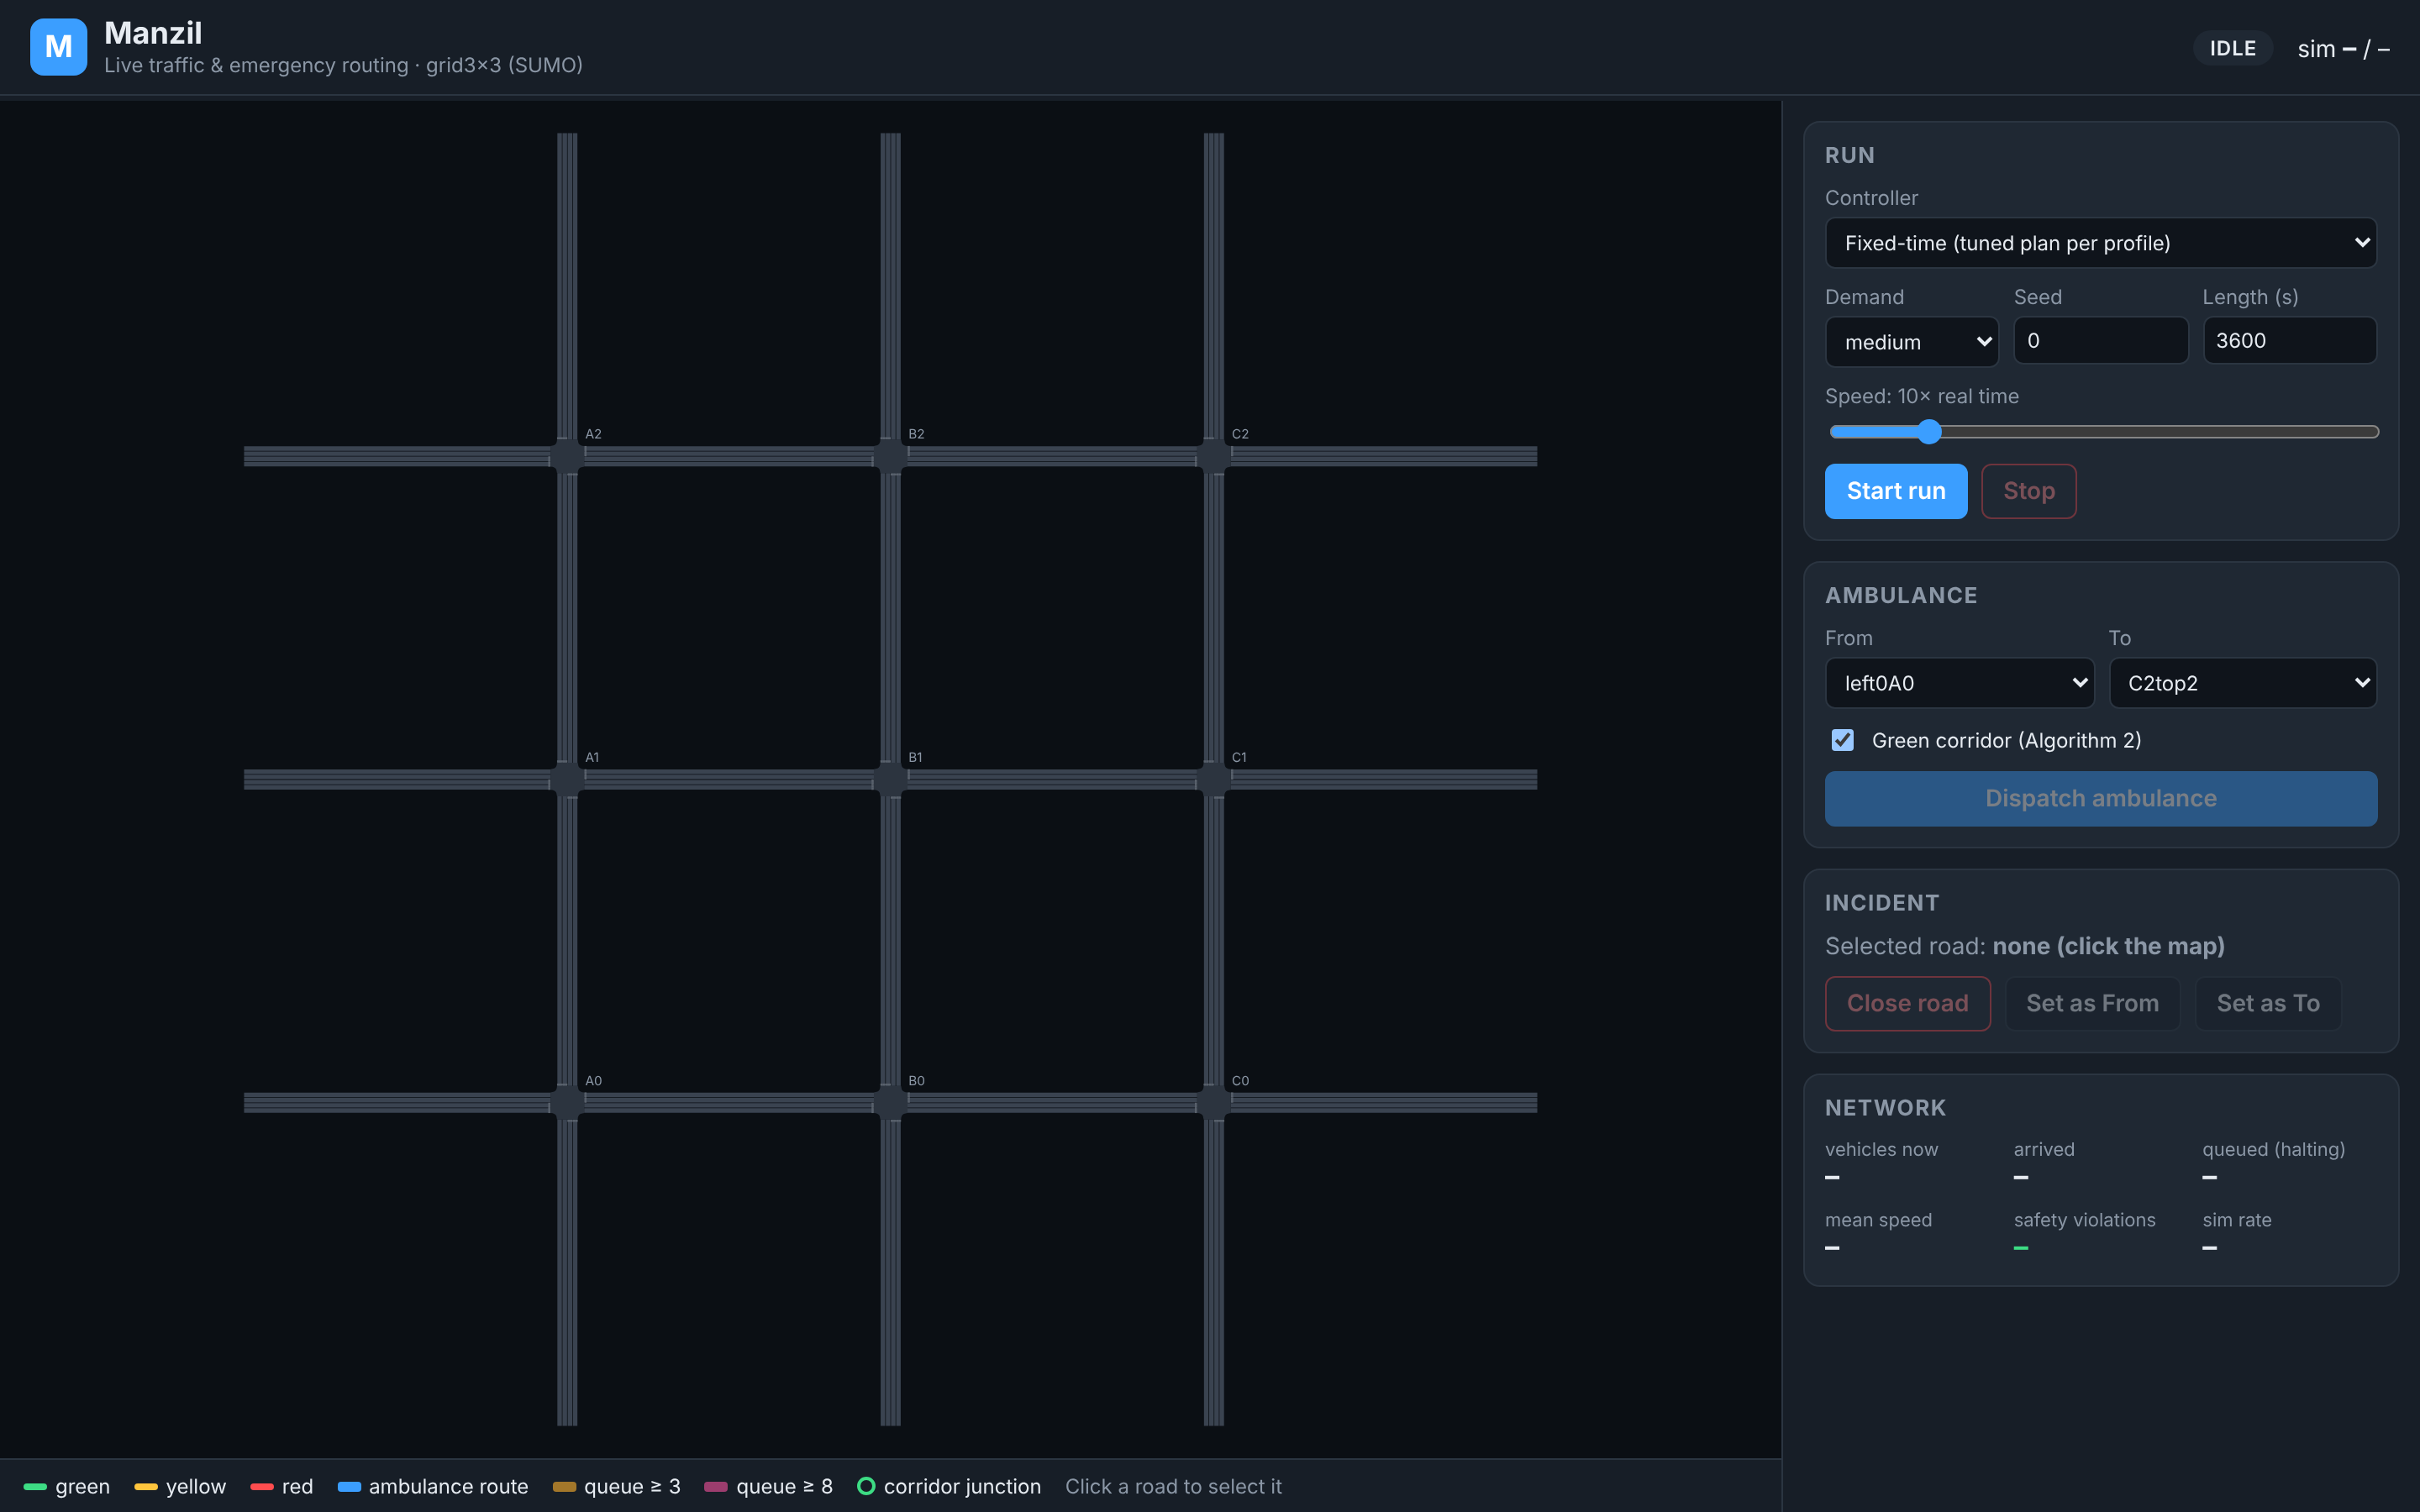
\includegraphics[width=0.92\textwidth]{figures/results/dashboard_01_idle.png}
\caption{Dashboard before a run, with the network drawn from the SUMO file}
\label{fig:manual-idle}
\end{figure}

\section{Running a Simulation}

The \textsc{Run} panel selects the signal controller (fixed-time, adaptive, or DQN), the demand profile (light, medium, heavy, or uneven), the random seed, and the run length in seconds. \emph{Start run} launches SUMO; the header then shows the status, the simulation clock, and the chosen settings, and the speed slider changes how fast the run proceeds relative to real time. On the map, each signal is coloured green, yellow, or red at its stop line, small marks are vehicles, and roads are shaded amber when at least three vehicles queue and purple when at least eight queue, as explained in the legend at the bottom (Figure \ref{fig:manual-running}). \emph{Stop} ends the run; its records are written to a run folder under \path{runs/live/}.

\begin{figure}[htbp]
\centering
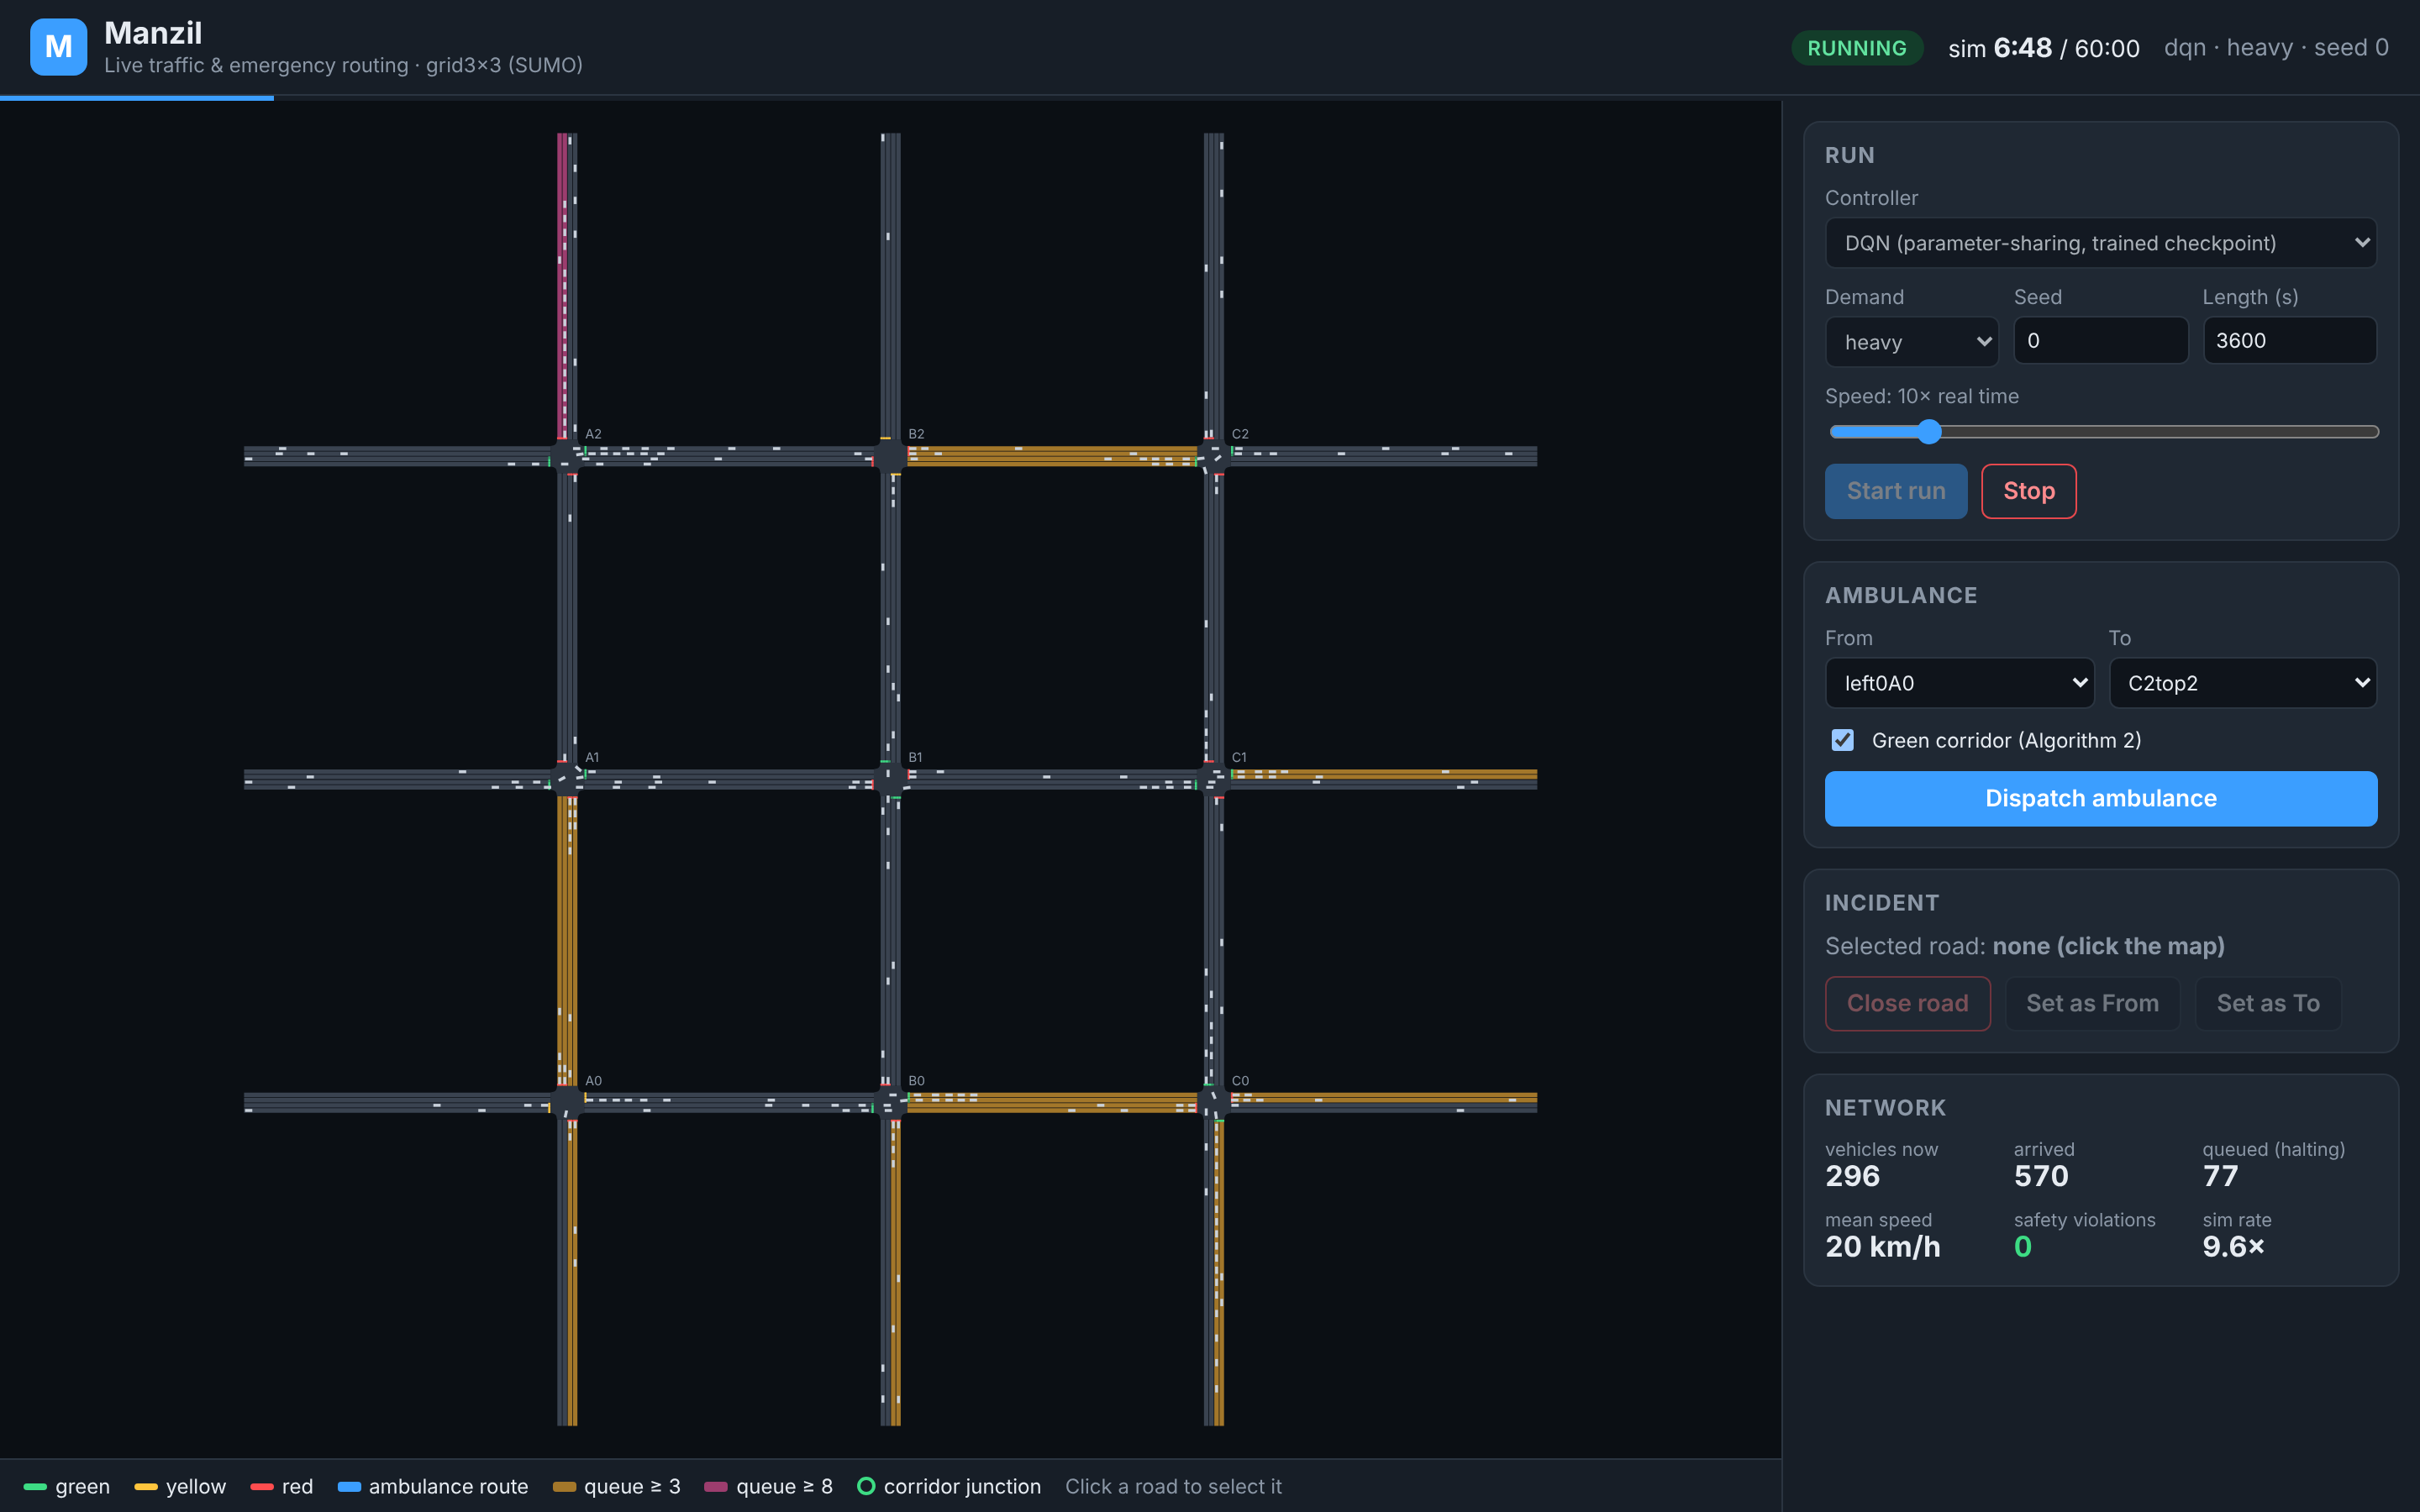
\includegraphics[width=0.92\textwidth]{figures/results/dashboard_02_running_dqn_heavy.png}
\caption{Running a heavy-demand simulation with the DQN controller}
\label{fig:manual-running}
\end{figure}

\section{Dispatching an Ambulance and Closing a Road}

The \textsc{Ambulance} panel selects the origin and destination roads and whether the green corridor is used. \emph{Dispatch ambulance} inserts the ambulance and computes its first route, which is drawn in blue. The panel then shows the mission status, the route version and what caused it, the ambulance's current road, speed, and number of stops, and the corridor state of each junction it is using, with a log of corridor events. Junctions held for the ambulance are marked with a ring. Only one ambulance can be active at a time.

To test rerouting, a road is selected by clicking it on the map and closed with the \textsc{Incident} panel. A closed road is marked with a red cross. If it lies on the ambulance's remaining route, a new route version with the trigger ``closure'' appears at once, and corridor requests that no longer lie on the route are cancelled (Figure \ref{fig:manual-closure}). When the ambulance reaches its destination, the mission status changes to \textsc{Arrived} and the panel shows its response time next to the free-flow time (Figure \ref{fig:manual-arrived}).

\begin{figure}[htbp]
\centering
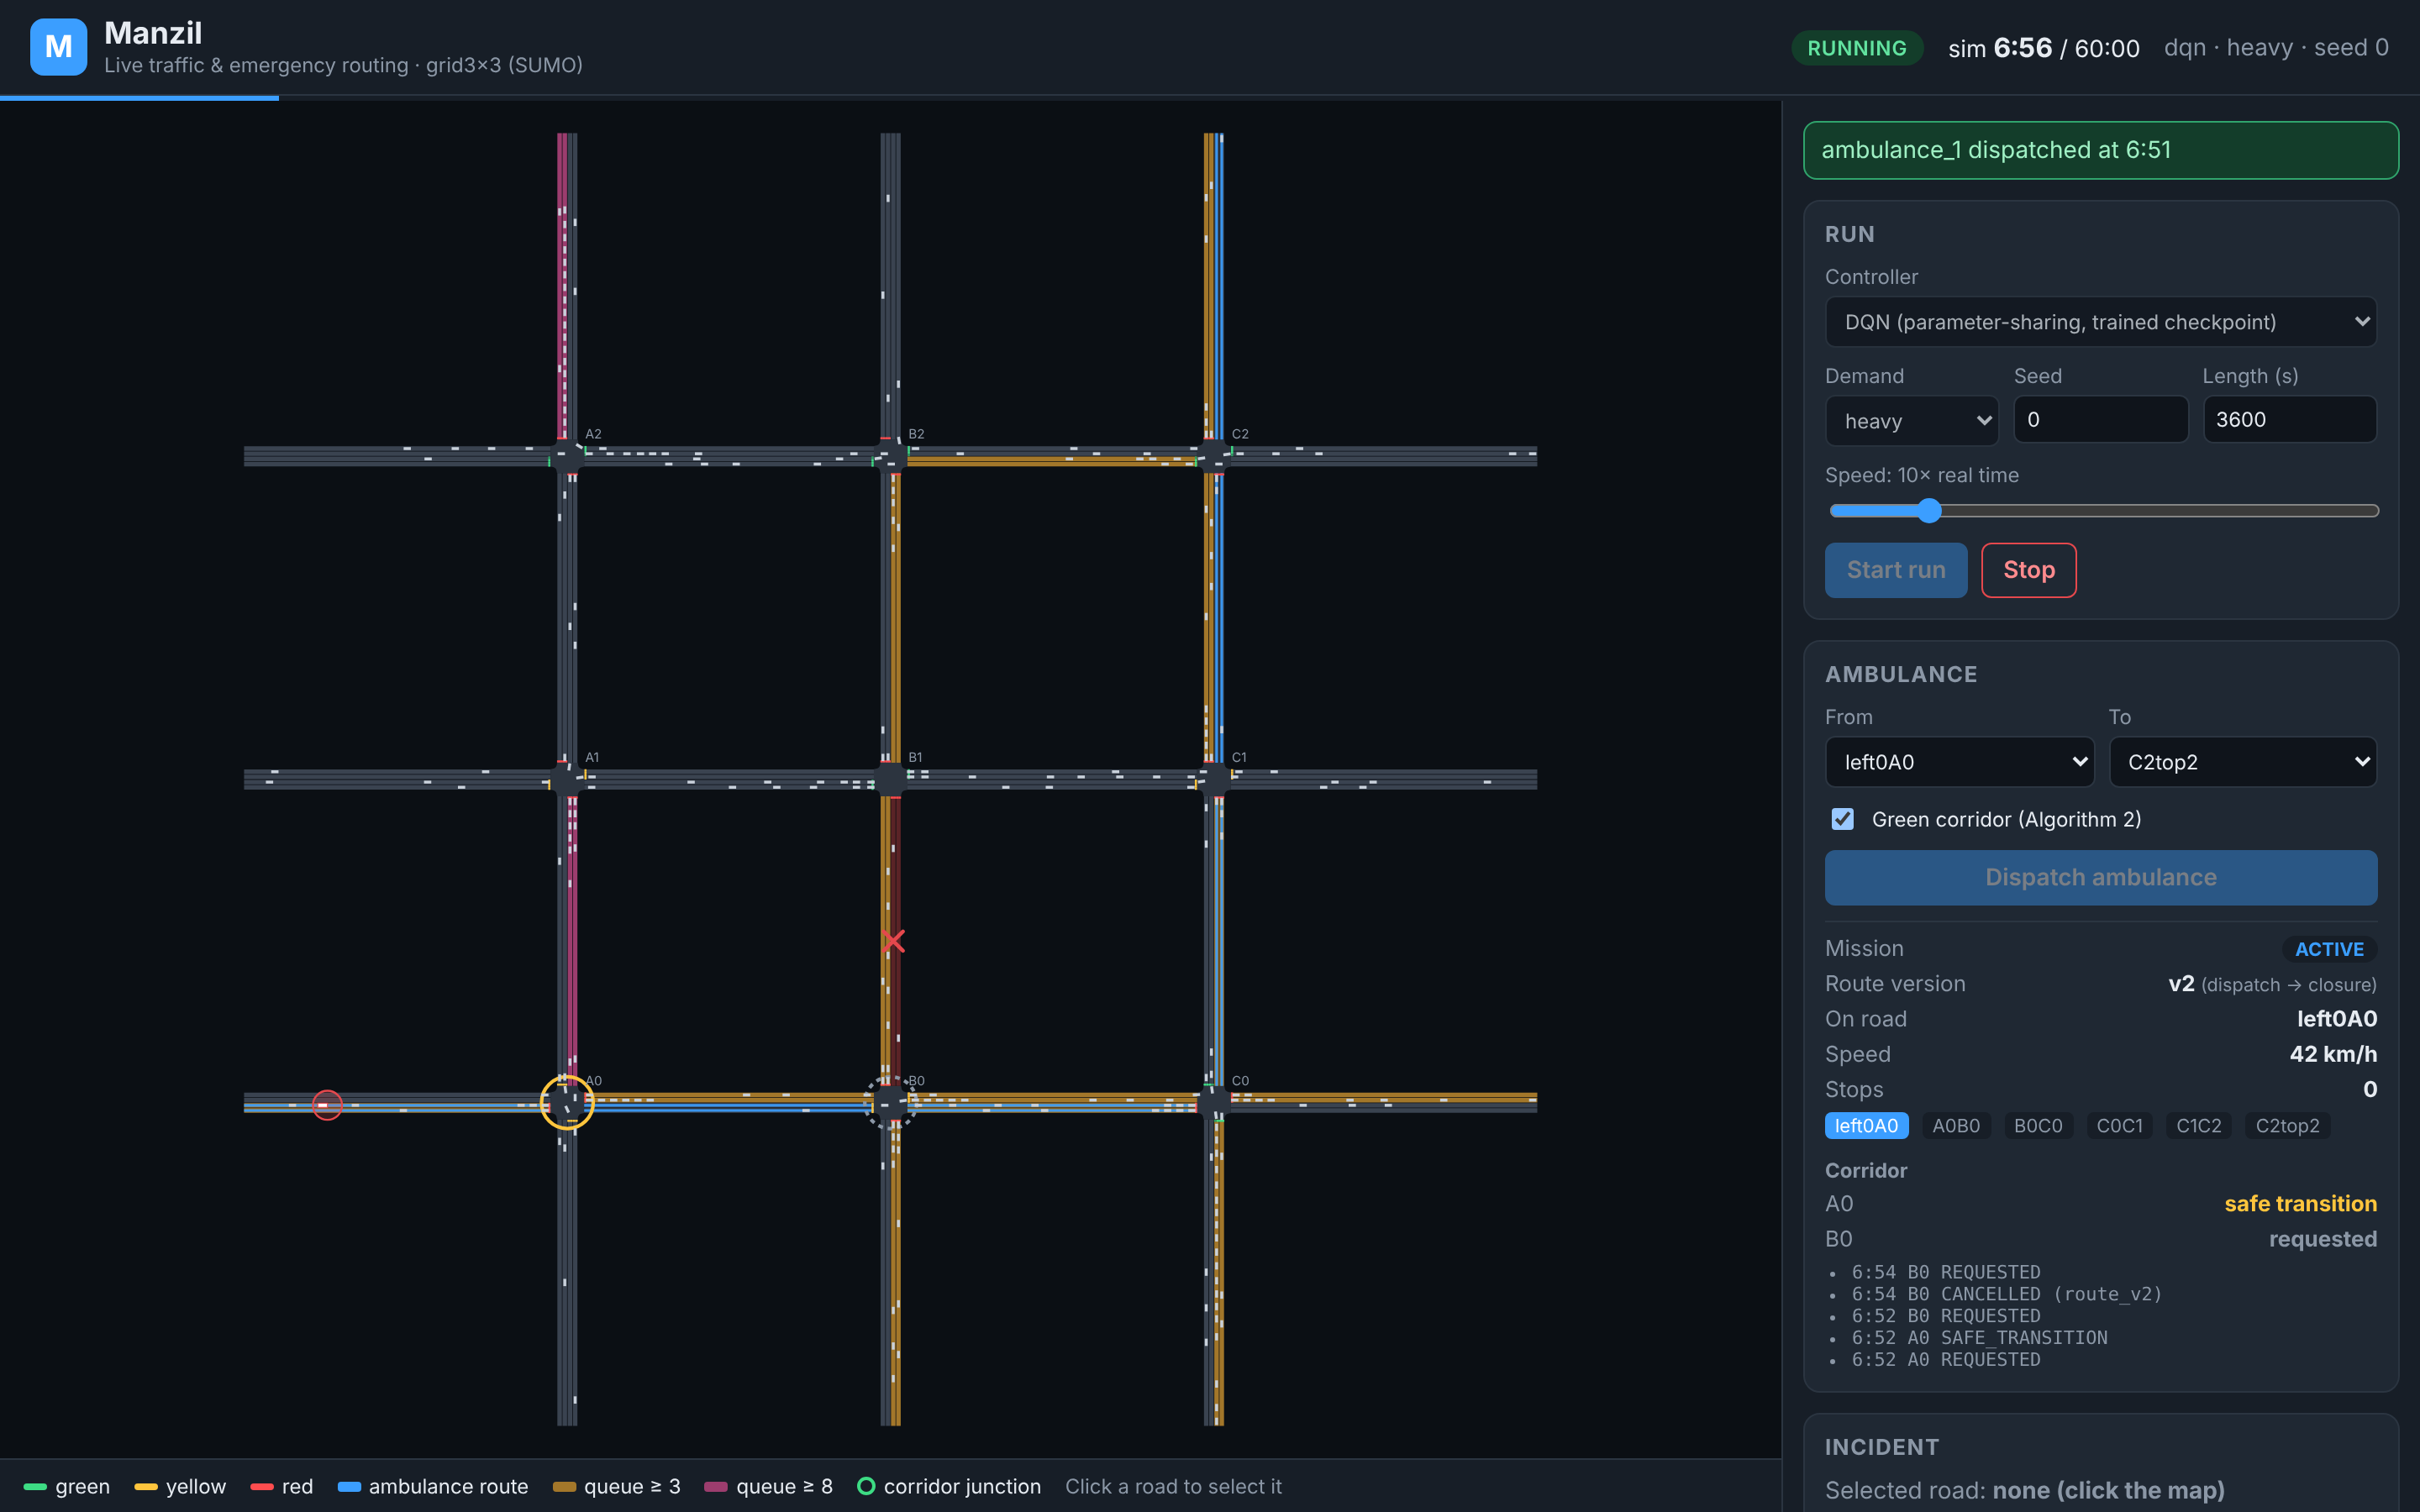
\includegraphics[width=0.92\textwidth]{figures/results/dashboard_03_closure_reroute.png}
\caption{A road closed on the route: route version 2 avoids it and the corridor requests are updated}
\label{fig:manual-closure}
\end{figure}

\begin{figure}[htbp]
\centering
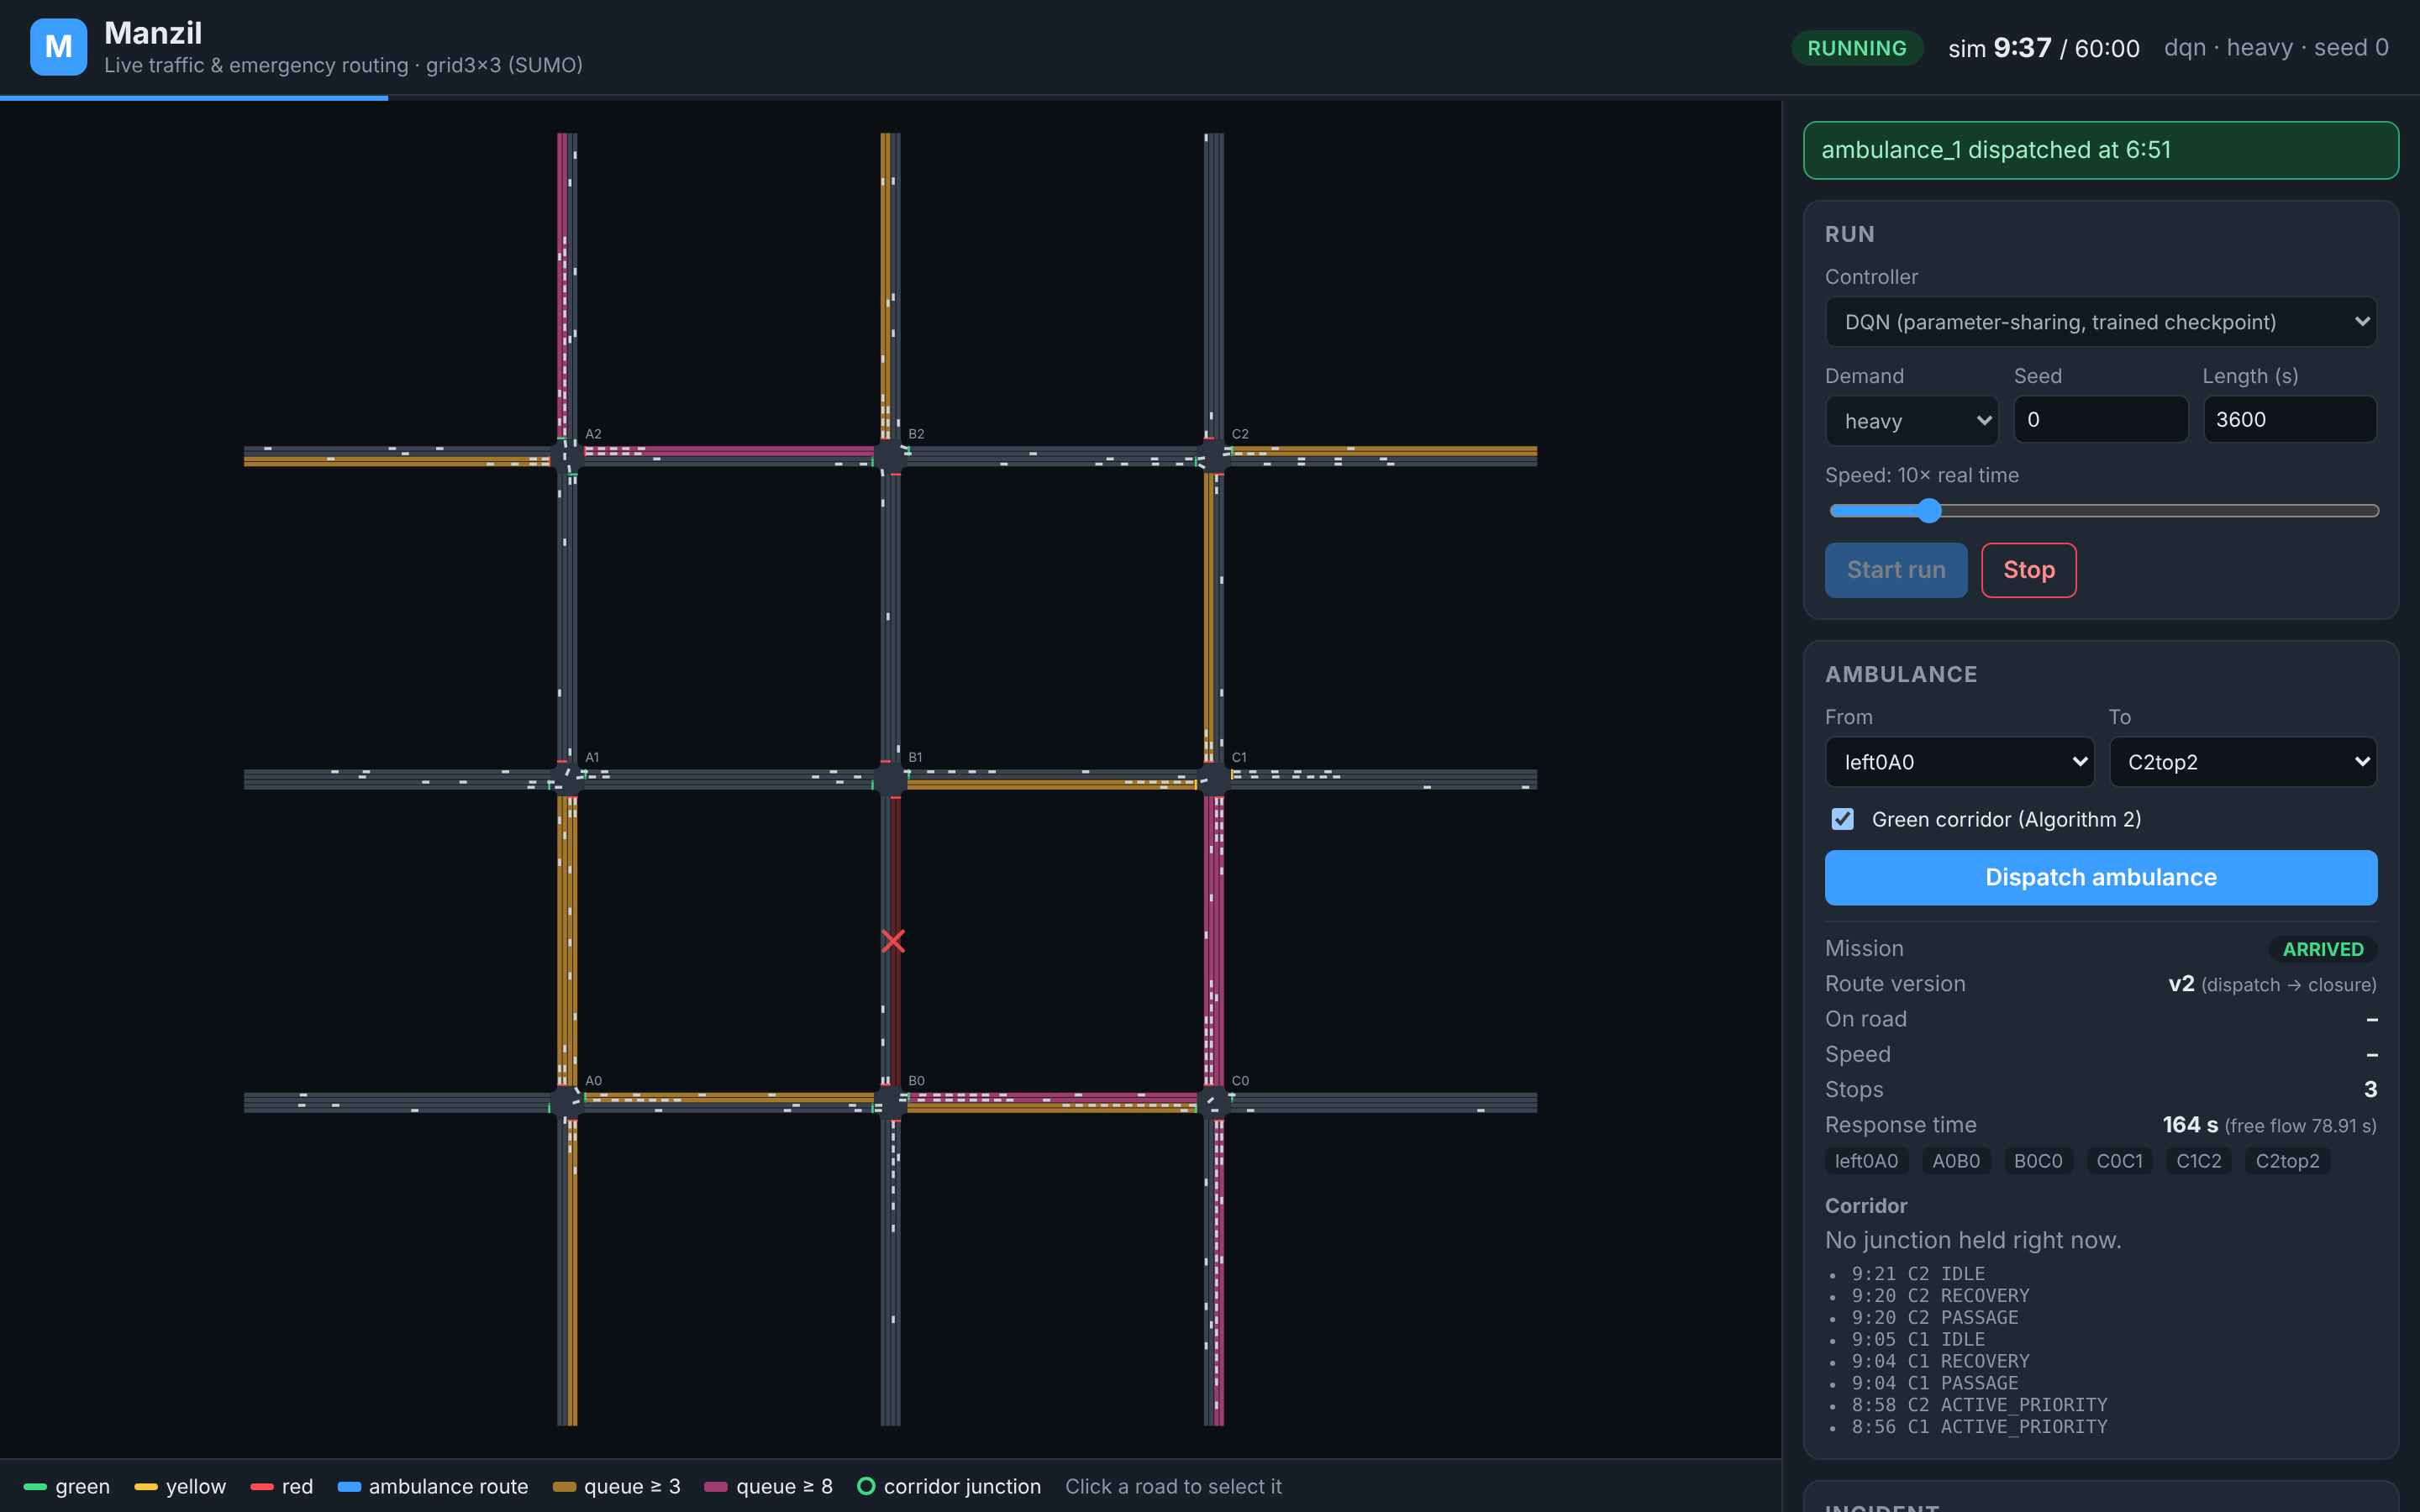
\includegraphics[width=0.92\textwidth]{figures/results/dashboard_05_arrived.png}
\caption{Mission arrived, with response time, stops, and the corridor event log}
\label{fig:manual-arrived}
\end{figure}

\section{Running the Experiments}

The controlled experiments are run from the command line rather than the dashboard, because they need many seeded runs. Table \ref{tab:manual-commands} lists the main commands; each writes its run folders and a summary into the given output folder. A complete list, including the vision jobs on Kaggle, is in the repository's README file.

\begin{table}[htbp]
\centering
\caption{Commands for repeating the experiments}
\label{tab:manual-commands}
\begin{tabularx}{\textwidth}{p{0.30\textwidth}Y}
\toprule
\textbf{Task} & \textbf{Command (after \texttt{python -m})}\\
\midrule
One run & \path{manzil.experiments.runner --profile medium --seed 0}\\
Controller comparison & \path{manzil.experiments.batch --arms fixed_time adaptive dqn --seeds 0 1 2 3 4 --out results/phase4/comparison}\\
Comparison statistics & \path{manzil.experiments.compare results/phase4/comparison/results.csv}\\
Routing and corridor & \path{manzil.experiments.emergency_study --seeds 0 1 2 3 4 --out results/phase3}\\
DQN training & \path{manzil.experiments.train_dqn --episodes 200 --out models/dqn/grid3x3}\\
Tests & \path{pytest}\\
\bottomrule
\end{tabularx}
\end{table}

\section{Conclusion}

The prototype is installed with a few commands and operated from one browser page: a run is started with a chosen controller, demand, and seed, an ambulance is dispatched between two roads, and a road can be closed to trigger rerouting while the corridor state is shown live. The same experiments as in Chapter \ref{ch:results} can be repeated from the command line. The full five-screen interface of Section \ref{sec:gui} is planned for FYP-II.
